%\documentclass[final, 2p]{elsarticle}
%\documentclass[review]{elsarticle}
\documentclass[graybox]{svmult}
%\documentclass[graybox]{svmult}

\usepackage{graphicx}
\usepackage[tight,footnotesize]{subfigure}
\usepackage{amsmath}
\usepackage{amssymb}
\usepackage{flushend}

\usepackage{pdflscape}
\usepackage{afterpage}
\usepackage{capt-of}% or use the larger `caption` package
\usepackage{algorithm}
\usepackage{algpseudocode}
\usepackage{xcolor,colortbl}
\let\proof\relax
\let\endproof\relax
\usepackage{amsthm}
\usepackage{amssymb}
\usepackage{mathrsfs}


\usepackage{url}
\usepackage{array}
\usepackage{paralist}
\usepackage{multirow}
\usepackage{tabularx}
\usepackage{color}

\newcommand{\N}{\mathbb{N}}
\newcommand{\R}{\mathbb{R}}

\newcommand{\blue}[1]{\textcolor{blue}{#1}}
\newcommand{\red}[1]{\textcolor{red}{#1}}
\newcommand{\magenta}[1]{\textcolor{magenta}{#1}}


\usepackage{setspace}
\setstretch{0.97}

\begin{document}

\title*{Towards Efficient Selective In-Band Network Telemetry Report using SmartNICs}


\author{Ronaldo Canofre, Ariel G. Castro, Arthur F. Lorenzon, Fábio D. Rossi, Marcelo C. Luizelli}

\authorrunning{Canofre et al.}
\institute{Ronaldo Canofre, Ariel G. Castro,  Arthur F. Lorenzon, Marcelo C. Luizelli \\Federal University of Pampa (UNIPAMPA) \at Alegrete, Brazil, \email{
{canofre, ariel.aluno , arthurlorenzon, marceloluizelli}@unipampa.edu.br}
\and Fabio D. Rossi\\ Federal Institute Farroupilha (IFFAR) \at Alegrete, Brazil, \email{fabio.rossi@iffarroupilha.edu.br}
}


\maketitle

\begin{abstract}\\
In-band Network Telemetry (INT) is a promising network monitoring approach that allows broad and fine-grained network visibility. However, when a massive volume of telemetry data is reported to an INT collector, there might overload the whole network infrastructure, while still degrading the performance of packet processing at the INT sink node. As previously reported in the literature,  programmable devices -- in particular, SmartNICs -- have strict constraints in terms of processing and memory. In this work, we propose to design and implement a lightweight Exponentially Weighted Moving Average based mechanism inside the SmartNIC data plane in order to assist the decision-making process of reporting INT data. By evaluating our solution in state-of-the-art SmartNICs, we show that our proposal can decrease the number of nonessential telemetry data sent to INT collectors by up to 16X compared to the de-facto INT approach while presenting minor overhead in terms of packet latency.

\end{abstract}


\section{Introduction}
\label{sec:introduction}

In-band Network Telemetry is a promising near real-time network monitoring approach~\cite{tpp-jeyakumar2014, 8526824, infocom19-pathplanning} that enables wide and fine-grained network visibility. In a nutshell, INT consists of instrumenting the collection of low-level network monitoring statistics directly from the data plane -- allowing network operators/monitoring applications to be fed with an unprecedented level of information. Examples of such in-network statistics include data plane metadata (e.g., per-packet processing time, or queue utilization), and/or custom-made ones (e.g., network flow inter-packet gap~\cite{SIGCOMM-2020-poster}). Over the last years, INT has been successfully applied to a series of use cases~\cite{9687464}, including the identification of short-lived network behaviors~\cite{10.1145/3265723.3265731} and network anomalies~\cite{comml-hohemberger-2019}.

In the classic hop-by-hop INT specification (i.e., INT-MD (eMbed Data)\footnote{INT specification: \url{https://github.com/p4lang/p4-applications/blob/master/docs/INT_v2_1.pdf}}), an INT source node embeds instructions into production network packets typically using either unused header fields (e.g., IPv4 options) or by re-encapsulating the network traffic (e.g., using INT encapsulation). Then, INT transit nodes embed metadata to these packets according to the instructions given by the INT source. Last, an INT sink node strips the instruction out of the packet and sends the accumulated telemetry data to an INT collector. Figure 1 illustrates the whole INT procedure. In this example, a packet from network flow $f_1$ is used to collect INT data from forwarding devices $A$ to $F$. Recently, investigations have made the first efforts to efficiently orchestrate how INT metadata are collected by network packets~\cite{infocom19-pathplanning, IntOpt-8761722, comml-hohemberger-2019, 9330755} in order to increase network visibility and timely detect network events. That includes, for instance, selecting the appropriate network flows/packet to collect the right network telemetry metadata in the network infrastructure. This problem has been proved to be NP-hard since packets might have different spare capacities (e.g., limited by the MTU data link)~\cite{JISA2019-int}. 

Despite these efforts, little has yet been done to efficiently and wisely report the collected telemetry data to an INT collector~\cite{9525085}. In the case where all the telemetry data is reported to an INT collector, there might lead to \textit{(i) an excessive usage of network links between the INT sink and the INT collector}. For instance, if we consider a 10 Gbit/s network link sending $64$-Bytes packets (i.e.,  $14.88$ Mpps) and collecting 1 Byte per INT node transit along the way, the volume of network traffic needed to be reported per second would be $118$ Mbit $*$ hops (path length). In fact, this volume of reported data can increase substantially if we assume the canonical reference architecture for programmable devices\footnote{\url{https://github.com/p4lang/p4c/blob/main/p4include/v1model.p4}} where each device has at least 30 Bytes of metadata; \textit{(ii) performance degradation on packet processing capabilities at the INT sink} due to the usage of packet cloning/recirculation primitives inside the data plane. To send the network packet to the INT collector (or part of it), programmable devices have to rely on packet recirculation/cloning primitives to duplicate the packet -- which dramatically reduces the performance in terms of throughput and latency~\cite{aina2021}; and \textit{(iii) the overwhelm of the INT collector application} with INT data packets.

\begin{figure}[t]
\centering
        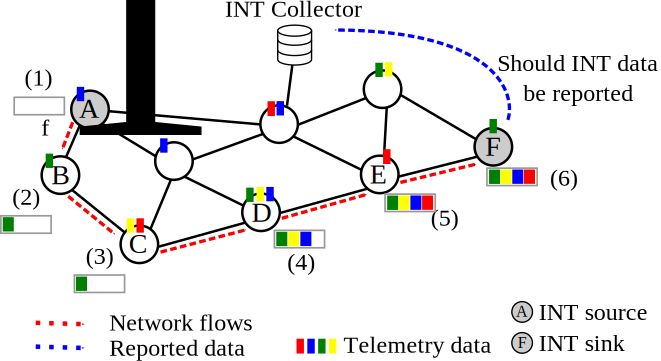
\includegraphics[scale=0.4]{aina-img/telemetry-canofre-aina.pdf}
        \caption{Overview of the problem.}
        \label{fig-problem-overview}
\end{figure}

To fill in this gap, in this work we propose a selective INT report mechanism entirely implemented using a SmartNIC. As previously reported by~\cite{aina2021}, programmable devices have stringent constraints in terms of processing capabilities (e.g., lack of floating-point operations) and memory usage limitations. We assume that the INT sink node is on top of a SmartNIC and, therefore, the decision whether report telemetry data or not is upon the NIC. Our proposed mechanism utilizes a lightweight Exponentially Weighted Moving Average inside the data plane. For that, we implemented it using P4 language and Micro-C routines to allow more complex operations inside the data plane. By performing an extensive performance evaluation using SmartNICs, we show that our proposed approach can reduce the amount of non-important telemetry data sent to INT collector by up to 16X (when compared to the Classical INT), while introducing negligible overhead in terms of packet latency.

The main contributions of this paper can be summarized as:

\begin{itemize}
    \item an in-network mechanism implemented in state-of-the-art SmartNICs to wisely decide when to report INT metadata;
    \item a discussion of current limitations on implementing in-network computing in SmartNIC architectures; and
    \item an open-source code in order to foster reproducibility. 
\end{itemize}

The remainder of this paper is organized as follows. In Section~2, we describe the SmartNIC architecture used in this work. In Section 3, we introduce our proposed approach. In Section 4, we discuss the obtained results. In Section~5, we overview the recent literature regarding in-band network telemetry, and. Last, in Section~6, we conclude this paper with final remarks.


%Due to the rich spectrum of benefits behind INT, there is increasing attention from the networking ecosystem fostered  by the rapid adoption of programmable data planes and domain-specific networking description languages (e.g., P4~\cite{p4-ref}).



%Since its inception, INT has been successfully applied to a series of use cases, including the identification of short-lived network behaviors and network anomalies. 
%Due to the rich spectrum of benefits behind INT, there is increasing attention from the networking ecosystem fostered  by the rapid adoption of programmable data planes and domain-specific networking description languages (e.g., P4~\cite{p4-ref}).
%In short, INT consists of instrumenting the collection of low-level network monitoring statistics directly from the data plane. Probing packets consists of specially crafted packets that instruct programmable forwarding devices to collect telemetry data. Figure~1 illustrates the entire INT process. In the first step, probing packets are generated aiming at instrumenting the collection of telemetry data along a given path. For example, the red flow (i.e. $f_1$) -- that is routed through the forwarding devices $A$, $E$, $F$, $G$, $H$, and $I$ -- carries instructions to collect telemetry data from devices $A$ to $H$. In the second step, the collected telemetry data is extracted and reported to an INT collector. 
%In short, INT consists of instrumenting the collection of low-level network statistics directly from the data plane. In the classic hop-by-hop INT (a.k.a INT-MD (eMbed Data)\footnote{INT specification: \url{https://github.com/p4lang/p4-applications/blob/master/docs/INT_v2_1.pdf}}), an INT source node embeds instructions into  production network packets. Then, INT transit nodes embed metadata while an INT sink node strips the instruction out of the packet and sends the accumulated telemetry data to an INT collector.


%\textbf{OLD from here!}


%context
%Programmable Data Planes (PDP) is a mainstream technology that has been recently redesigning the networking domain. PDP allows to (re)define the behavior of network devices (e.g., programmable routers and SmartNICs), allowing to deliver specialized packet processing mechanisms~\cite{p4-ref}. Recent advances in data plane programmability have enabled offloading typical control plane applications to the data plane (e.g., machine learning algorithms~\cite{xiong2019switches}, routing~\cite{8737398-infocom}, or network monitoring~\cite{9330755, 8865384, aina2020-rumenigue}). On shifting the operation of these applications to the data plane, it brings the benefit to process every single packet and react to network conditions in the order of nanoseconds, with minimum control plane intervention.
%
%Despite that, data plane operation might become complex -- and the complexity comes at a price: \emph{lower throughput and higher latency}. 


%Current SmartNIC architectures (e.g., \cite{netronomeArc}) do not limit the number of operations performed by the data plane in a single pipeline stage. For example, a PDP application could trigger the read and write of an unbounded number of registers in a given stage of the packet processing pipeline. Yet, the same application could recirculate the ingress packet multiple times to mimic a loop-based mechanism. These are straightforward examples of simple operations commonly used by more complex PDP applications (e.g., in-network clustering~\cite{xiong2019switches}). Therefore, understanding the current performance limitations of existing SmartNICs is paramount to the design of efficient PDP applications.


%evaluate  different  P4  constructs  and  their  impact  onthe packet processing latency. They gradually increase the complexity of aSmartNIC  pipeline  (i.e.,  including  parser,  control  blocks,  and  deparser)  toidentify the most influential variables and present a generalized estimation

%A recent study~\cite{harkous2019towards} has made the first effort to understand the existing limitations of SmartNICs. Harkous et al.~\cite{harkous2019towards} have focused on evaluating the performance of general PDP metrics such as parsers, control blocks, and header modifications in P4 programs. Despite this effort, no study has yet thoroughly evaluated key building blocks of complex P4 programs (e.g., registers, cryptography functions, or packet recirculation) -- which are essential for most recent P4 applications.
%
%To fill in this gap, we perform an extensive performance evaluation of SmartNICs to understand and quantify PDP application primitives and existing limitations. We focus our evaluation on measuring the performance in terms of latency and throughput for a variety of packet sizes (from 64B to 1500B) when (i) operating multiple registers of different sizes/widths (e.g., used to implement bloom filter alike structures~\cite{hhh-sigcomm}), (ii) matching on multiple tables in the ingress and egress pipeline (e.g., used to implement machine-learning algorithms~\cite{xiong2019switches}), (iii) performing packet recirculation (e.g., used to implement IoT data desegregation~\cite{WANG201998}), and (iv) using cryptography functions and arithmetic operations. Results show that network throughput can degrade up to 8X, while latency can increase as much as 80X when performing memory-intensive operations in the data plane. The main contributions of this paper can be summarized as:

%\begin{itemize}
%    \item an in-depth performance evaluation of SmartNICs;
%    \item a discussion of current limitations in SmartNIC architectures; and
%    \item an open-source code of all experiments in order to foster reproducibility. 
%\end{itemize}

%The remainder of this paper is organized as follows. In Section~2, we describe the SmartNIC architecture used in this work. In Section~3, we overview the recent literature regarding PDP applications and performance evaluation. In Section 4, we present and discuss the obtained results and, in Section~5, we conclude this paper with final remarks. 

\section{Background} 

Cutting-edge programmable NICs (named SmartNICs) rely their architectures either on (i) multi-threaded, multi-core flow processor units or (ii) on FPGAs (Field Programmable Gate Arrays) to meet the increasing and strict demand. We concentrate our analysis on the general architectural elements of the Netronome SmartNIC architecture~\cite{netronomeArc} -- which is used afterward in our performance experiments -- and rely on a multi-core architecture. 

\begin{figure}[!htb]
\centering
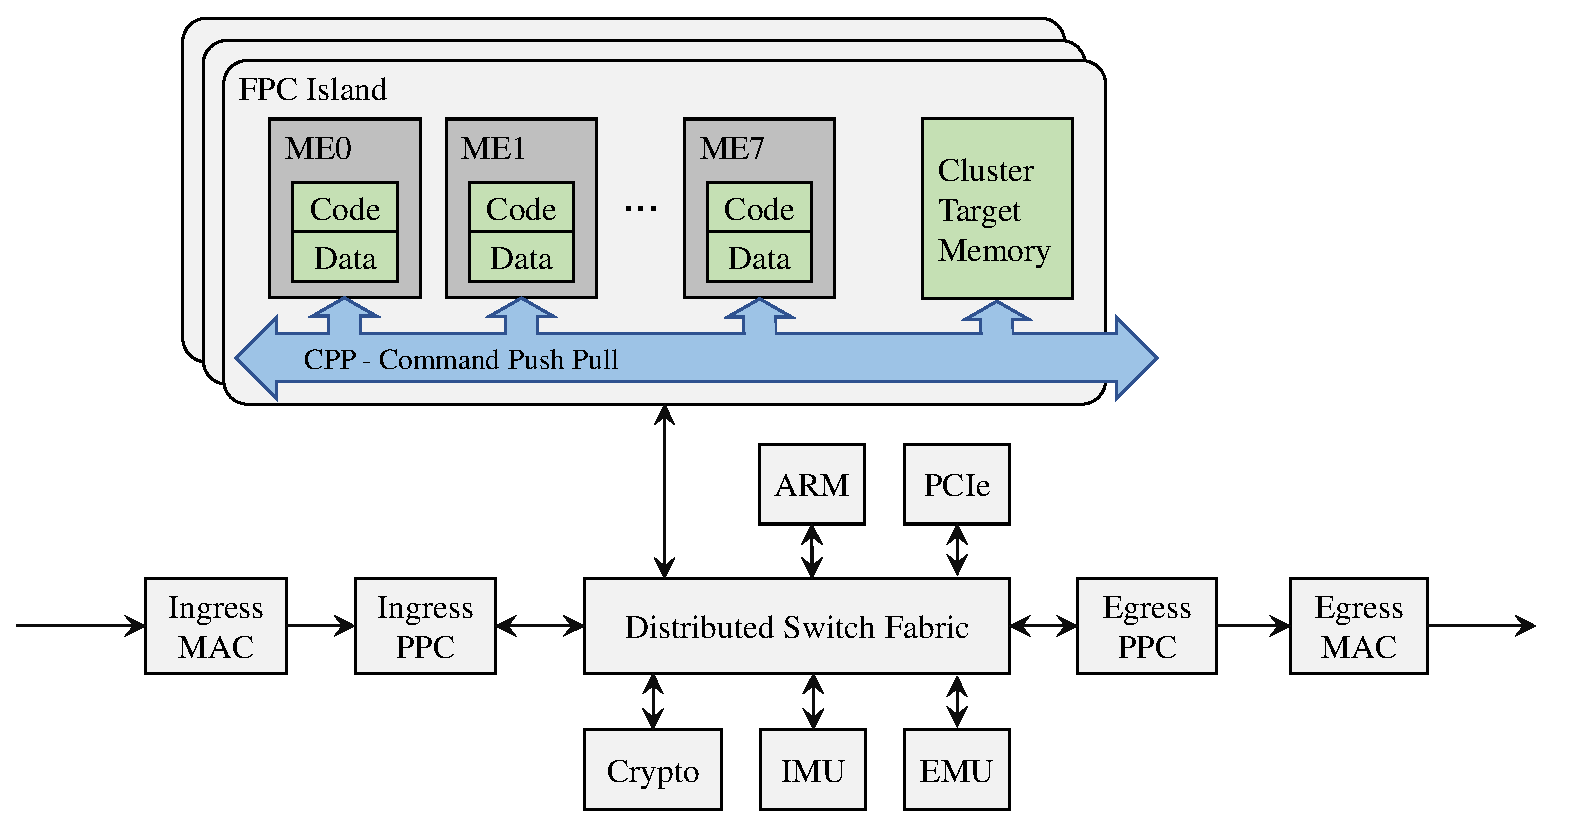
\includegraphics[scale=0.3]{img/architecture.eps}
\caption{An overview of the Netronome SmartNIC architecture~\cite{aina2021}.}
\label{fig-architecture}
\end{figure}

The SmartNIC Netronome NFP4000 architecture manages its flow processing cores (FPC) in multiple islands (Figure~\ref{fig-architecture}). Each FPC includes eight Micro Engines (MEs) as a particular processor keeping its own instruction store (\textit{code}) and local memory (\textit{data}). 
Therefore, every ME in the architecture can run code with all other MEs in parallel. To support this feature, each ME holds 8 threads that can be used for cooperative multithreading in the manner that,  at any given moment, at most, one thread is executing code from the same program. It means that each FPC handles at most eight parallel threads at 1.2Ghz (one thread per ME). In each FPC, local memory comprises 32-bit registers, shared between all eight threads. Such registers are separated into: (\textit{i}) general-purpose registers (256 32-bits registers) -- used by default to store any register of up to 32-bits size; (\textit{ii}) transfer registers (512 32-bits registers) -- used for copying register over the interconnection bus (e.g., from or to other FPCs or memories); (\textit{iii}) next-neighbor registers (128 32-bits registers) -- used mostly to intercommunicate with adjacent FPCs; and (\textit{iv}) local memory (1024 32-bit registers) -- which is a little bit slower than general register. When there is a demand for more memory than available space in local FPC registers, variables are automatically and statically assigned to other in-chip memory hierarchies. Further, there are other sorts of memory available to FPCs: (\textit{i}) Cluster Local Scratch (CLS) (20-50 cycles); (\textit{ii}) Cluster Target Memory (CTM) (50-100 cycles); (\textit{iii}) Internal Memory (IMEM) (120-250 cycles); and (\textit{iv}) External Memory (EMEM) (150-590 cycles). For further details, the interested reader is referred to~\cite{netronomeArc}. 

As packets are acquired from the network, an FPC thread picks up the packets and processes them. Extra threads are assigned to new packets as they arrive. For example, the SmartNIC NFP-4000 supports up to 60 FPCs, which enables the process of up to 480 packets simultaneously. The SmartNIC allows to program it directly using Micro-C language (i.e., a subset of C language) or using high-level domain-specific languages such as P4~\cite{p4-ref}. The code is then compiled and statically assigned to a particular subset of FPC. 

%In resume, the local memory register is used for data used in every packet. The CLS is used for data required for most packets and small shared tables. The CTM is used for packet headers and management between other sub-systems. IMEM is used for packet bodies and medium-sized shared tables. Finally, EMEM is used for extensive shared tables. 




%old:
%The SmartNIC architecture is illustrated in Fig. \ref{fig-architecture}. It organizes its flow processing cores (FPC) in multiple islands. Each FPC runs at most 8-threads in parallel at 1.2Ghz. However, in-chip islands do not follow the same architectural design. For example, some islands may contain mostly FPC processing units. Others, in turn, may have fewer processing units but other functionalities such as PCIe interfaces or crypt sub-systems.
%
%The FPC is a 32-bit machine and, therefore, all of its internal registers and local memory are formed from 32-bit words. FPCs follow a Harvard Architecture and therefore code and data occupy different memories. Usually, 4K bytes are shared between all 8 threads for data and a reserved memory of 8K instructions for the coding store. Every thread on an FPC runs the same program, held in the single code store shared by all the threads.
%
%Local memory in each FPC  is composed of a set of 32-bit registers, shared between all 8 threads. These registers are divided into (i) general-purpose registers (256 32-bits register) -- used by default to store any register of up 32-bits size; (ii) transfer registers (512 32-bits registers) -- used for copying register over the interconnection bus (e.g., from or to other FPCs or memories); (iii) next-neighbor registers (128 32-bits register) -- used mainly to communicate with neighboring FPCs; and last (iv) local memory (1024 32-bit register) -- which is a little bit slower than general register (3 cycles access, instead of just 1 cycle). When there is a need for more memory than available space in local FPC registers, variables are automatically and statically allocated to other in-chip memories hierarchies. 
%
%There are four other kinds of memory which are available to FPCs: (i) Cluster Local Scratch (CLS) (20-50 cycles); (ii) Cluster Target Memory (CTM) (50-100 cycles); (iii) Internal Memory (IMEM) (120-250 cycles); and (iv) External Memory (EMEM) (150-590 cycles). In summary, the local memory register is used for data that is used for every packet. Then, the CLS is used for data that is needed for most packets and small shared tables. The CTM is used for packet headers and coordination between other sub-systems. Then, IMEM is used for packet bodies and medium-sized shared tables. Finally, EMEM is used for large shared tables. 

%As packets are received from the network, an FPC thread picks up the packet and processes it. Additional threads are allocated to new packets as they arrive. For instance, the SmartNIC NFP-4000 supports up to 60 FPCs, each supporting up to 8 threads. Then, the device can process up to 480 packets simultaneously.


%Transfer registers. All data traveling over the CPP bus to or from CLS, CTM, IMEM, or EMEM must go through a transfer register. Just to emphasize this: CPP data cannot come directly from or go directly to general-purpose registers. It must instead go via transfer registers. There are 256 32-bit transfer-in registers, also known as “read registers”. These are used to receive data that arrives via a CPP Push operation. Several sequential registers can be transferred from the CPP bus in one Push operation. From ME code, these registers are read-only. They are shared between the 8 threads, so each thread has 32 transfer-in registers. There are also 256 32-bit transfer-out registers, also known as “write registers”. These are used to provide the data which is taken by a CPP Pull operation. Data from several sequential registers can be transferred onto the CPP bus in one Pull operation. From ME code, these registers are write-only. They are shared between the 8 threads, so each thread has 32 transfer-out registers. Transfer registers can in principle be indexed, but the ME hardware has only one transfer index register, shared between all threads, which makes generating code to use this index register slightly tricky. The compiler does not currently attempt to do this, and arrays that are indexed by values that vary at runtime cannot, therefore, be allocated to transfer registers.
%







\section{ETA: Early Network Telemetry Flow Analyzer Approach}
%apf eta 

In this section, we first define the model used by our proposed approach to decide whether or not network telemetry data is sent to an INT collector. Then, we describe how it is implemented in a SmartNIC and discuss existing limitations and challenges.

\subsection{Model and Problem Definition}

We consider that a programmable forwarding device $d \in D$ has $N \in \mathbb{N}^{+}$ available metadata to be collected by an INT-enabled packet $p$ and that such packet has a limited available capacity to carry up to $M \in \mathbb{N}^{+}$ of such $N$ items ($M \geq N$). For simplicity, we assume that all devices $D$ have the same telemetry information and that an INT-enabled packet $p$ can only collect telemetry data atomically, that is, it either collects all $N$ metadata from $d \in D$ or none of them. Packet $p$ can only collect once the same subset of telemetry data from the device $d$. We assume that the INT source instructs the packet $p$ correctly according to a given algorithm (e.g., \cite{JISA2019-int}). 

Consider that a packet $p$ has collected $M' \subseteq M$ telemetry data along its routing path -- which comprises a subset of $D$ devices. When the packet $p$ gets to the INT sink node, the question to be answered is: \textit{should it be sent to the INT collector or not?} To answer this question, the INT sink node computes (i) a weighted average of metadata $M'$ collected by packet $p$ and (ii) an exponential weighted moving average. The former tends to weigh the collected telemetry data differently according to its importance. For instance, the processing time (or the queue utilization) metadata might be more important to be considered in the decision process than the packet size. In turn, the latter tends to keep in memory the observed behavior of the latest received telemetry information over time. 

Upon a received packet $p$ in the INT sink node, it extracts the $M'$ collected telemetry metadata and computes a weighted average per packet $A_p = \sum_{i = 1}^{M^{'}} w_i \cdot M_i$ (Eq. 1), where $w_i \in [0, 1]$ is the i-\textit{th} weight given to the telemetry data. We further assume that $\sum_{i = 1}^{M} w_i = 1$ and that $M_i$ corresponds to the i-\textit{th} collected data. Such individual averages $A_p$ are then summing up into a accumulated weighted average metric within a given time window $W$ (we discuss this design choice next). The time window $W$ is  defined for simplicity as a predefined number of packets. However, it can be extended to other metrics such as a time interval. 

Then, the accumulated weighted average of a given window $W$ is given by $A_w = \frac{\sum_{p = 1}^{W} A_p}{W}$ (Eq. 2). Similarly, the exponential weighted moving average is obtained by $A_e = \alpha \cdot A_w + (1 - \alpha) \cdot A_e$ (Eq. 3) where $\alpha \in [0,1]$ comprises the importance given by the elements obtained in the last window $W$ versus the historical knowledge maintained by the moving average $A_e$. Observe that higher values assigned to $\alpha$ prioritize the behavior on the latest window, while lower values prioritize the observed behavior over time. The decision-making process is made in a per-packet manner; however, the decision-making metrics (e.g., $A_e$) are updated in a time-window manner.


\subsection{Design and Implementation in a SmartNIC}


Figure~\ref{fig-overview} illustrates an overview of the proposed approach pipeline implementation. Our approach utilizes the reference V1Model architecture to programmable forwarding devices as the basis to implement/add such functionalities into the Netronome SmartNIC. Also, our approach is based on P4-16 and in Micro-C languages. 

Upon a packet is received by the SmartNIC, the packet is parsed accordingly. Our approach implementation resides just after the parsing step and the ingress pipeline (where the routing decision takes place), that is, in the egress pipeline. For this discussion, we assume that our forwarding device can process Ethernet frames and IP packets (or any known INT encapsulation protocol). Therefore, we omit the parsing steps since it is trivial and out of this work's scope. We then focused on the following up steps.   

\begin{figure}[t]
\centering
        \includegraphics[scale=0.38]{aina-img/apf-overview.pdf}
        \caption{Overview of the proposed P4+Micro-C pipeline approach.}
        \label{fig-overview}
\end{figure}

Our approach is implemented in the INT sink. Therefore, at this stage, all INT telemetry metadata has already been collected. The first steps of our approach consist of receiving the packet and extracting the telemetry data from it -- or, in some cases, collecting them directly from the data plane (this might happen when the INT sink node acts as an INT transit node as well). This corresponds to steps 1 and 2 in Figure~\ref{fig-overview}. The extracted data is then stored in a custom-made metadata header structure -- named \texttt{ETA} metadata struct. This structure comprises $M$ 32-bit structures and a 2-bit flag used to instruct the decision-making process. For instance, if a packet needs to be sent to the INT collector, this flag is used internally. In the Netronome architecture, the existing timestamps (\texttt{ingress\_timestamp} and \texttt{current\_timestamp}) are 48-bit words. However, most of the applications use only the least significant bits (the last 32 bits) since they account for nanosecond differences. Further, as discussed next, the Netronome architecture also limits the results of arithmetic operations to 32 bits words (and therefore, we cannot operate on 48-bits timestamps). After extracting telemetry data into the \texttt{ETA} struct, our implementation calls a Micro-C extern code to handle more complex operations inside the data plane (depicted in Figure~\ref{fig-overview-microc}). For instance, floating-point operations are not allowed in the P4-16 language reference, nor does the SmartNIC natively implement it. To allow the SmartNIC code to be partially written in P4 and Micro-C -- and more importantly, to exchange data between them -- we rely on \texttt{ETA} structs and internal P4 metadata to enable such real-time communications.

%
The Micro-C code starts receiving data from the P4 pipeline and locking up memory regions using a mutex (steps 1-3 in Figure~\ref{fig-overview-microc}).
%%%%%%%%%%
%\textcolor{blue}{due to the memory sharing adopted (discussed in more detail below)}.
%%%%%%%%%%
%That is necessary since our application shares memory regions between processors/threads to store the current window $W'$, as well as the current values of calculated averages (i.e. $A_e$ and $A_w$). 
%
Next, we calculate $A_p$  and $A_w$ according to Equation 1 and Equation 2, respectively. Figure~\ref{fig-overview-microc} illustrates these procedures in steps 4-7.  It is important to mention that neither the P4 reference architecture nor the Netronome support floating-point instructions. We implemented all these operations using fixed-point representation with 32 bits to surpass that limitation. In short, a fixed-point representation handles all real numbers as integers. The process scales up the numbers by multiplying by a constant factor $C$ and then performs the multiplications/division as a regular integer. Finally, the scaled-up result is scaled down appropriately. In our implementation, we have used a constant $C$ of 16 bits and performed the scale-up operation by applying a bit-shifting operation (i.e., $M'_i << 16$). After calculating $A_p$, we verify whether it is the case to send it out to the INT collector. We compare $A_p$ with the observed $A_e$ (which captures the historical behavior). In case the  $A_p$ packet value is higher than the dynamic $A_e$ one, we mark the packet to be sent out to the collector (steps 8-12 in Figure~\ref{fig-overview-microc}).
%%%%%

%\textcolor{blue}{
%Although the allocation of ​​variables can be performed dynamically by the compiler, following a controlled choice order, this process does not always present a satisfactory result for the processing of information. In the validation tests performed, both the dynamic approach and the definition of memories with lower latency (CLS and CTM), to store the current window $W'$, as well as the current values of calculated averages (i.e. $A_e$ and $A_w$), returned incorrect results in processing the information. Thus, in order to allow full access to data by all threads and MEs and also to obtain an exact result in the calculations performed, the shared information was statically allocated in the external memory of the EMEM which, despite having the highest latency among those available, did not have a relevant impact for the presented approach. Furthermore, due to the need to share memory regions between processors / threads to store information, in addition to the use of EMEM memory, it was also necessary to lock these regions, accomplished through the use of mutex.}


As previously mentioned, our approach performs per-packet decisions. However, we update the exponential weighted moving average $A_e$ at the end of a given window $W$. This is done because the average $A_e$ depends on $A_w$ -- and, the Netronome architecture does not allow arbitrary integer divisions (only by the power of 2 by performing bit-shifting -- for instance $M'_i >> 16$). Our approach verifies whether it reaches or not the end of a given window $W$ (step 14 in Figure~\ref{fig-overview-microc}). If so, then it updates the moving average $A_e$ (step 15-19 in Figure~\ref{fig-overview-microc}) according to Equation~3. Further, if it is the first time to reach the window $W$ (i.e., $W' == W$), then $A_e$ assumes a simple average of $A_w$ (step 20 in Figure~\ref{fig-overview-microc}). Then, the Micro-C sets the mutex down and allows other threads to use the blocked shared memory. Last, our Micro-C code returns the calculated values to the original P4 pipeline (step 22-23 in Figure~\ref{fig-overview-microc}). 

\begin{figure}[t]
\centering
        \includegraphics[scale=0.38]{aina-img/apf_micro_c.pdf}
        \caption{Overview of the proposed Micro-C routine.}
        \label{fig-overview-microc}
\end{figure}

Back in the P4 pipeline (Figure~\ref{fig-overview}), our approach clone and recirculate the packet $p$. The original packet is forwarded to its destination (step 13 in Figure~\ref{fig-overview}), while the cloned one is sent to the INT collector (step 12 in Figure~\ref{fig-overview}).

%To send the information back to the P4 pipeline, we use the same \texttt{ETA} struct as an auxiliary variable to store partial results (e.g.,  $A_p$). Then, we add $A_p$ to the partial sum of $A_w$, which will be calculated at the end of window $W$. The reason behind adopting this window strategy is because the Netronome Architecture does not support arbitrary division operations. In fact, it only supports division by a multiple of a power of 2.

%Then, we verify if our current window counting reaches the window size $W$. If so, it means that we need to calculate (in case it is the first) or recalculate our $A_e$ according to Equation 3. 


%\begin{figure}[t]
%\centering
%        \includegraphics[scale=0.55]{aina-img/apf_micro_c.pdf}
%        \caption{Overview of the proposed Micro-C approach.}
%        \label{fig-overview-microc}
%\end{figure}

%\subsection{Current Limitations of SmartNICs}

%Floating-point operations
%bit-shifting
%registers
%control-based structes
%metadata
\section{Performance Evaluation}

In this section, we perform a performance evaluation of our proposal mechanism using a Netronome SmartNIC. We start by describing our environment setup, followed by discussing the results.

\subsection{Environment Setup and Baseline Comparison}

\noindent\textbf{Setup.} Our environment setup consists of three high-end servers. Each server has an Intel Xeon 4214R processor with 32 GB RAM. One server is our Device Under Test (DUT) -- i.e., the server in which our solution (i.e., P4 program) is loaded -- and the other two are used for traffic generation. All servers have a Netronome SmartNIC Agilio CX 10 Gbit/s network device with two network interfaces, which are physically connected (i.e., each traffic generator is connected to the DUT directly). 
%
We use MoonGen\cite{moongen} as our DPDK\footnote{\url{https://www.dpdk.org/}} traffic generator. We instruct MoonGen using the Netronome Packet Generator\footnote{\url{https://github.com/emmericp/MoonGen/tree/master/examples/netronome-packetgen}}. In our experiments, we send 64B IPv4 packets at line rate (i.e., 10Gbit/s) with random source and destination prefixes. One of the traffic generator servers is used to send foreground network traffic, while the second is used to inject abrupt network traffic from time to time. This abrupt network traffic is generated with MoonGen to lead to a congested scenario. The experiment is run through 105 seconds, divided by time slots/epochs of 15 seconds each. We sent network traffic bursts in the following slots: 2\textit{nd} (15s-30s), 4\textit{th} (45s-60s), 6\textit{th} (75s-90s). In our experiments, the SmartNIC Netronome acts simultaneously as an INT transit and an INT sink. First, it collects internal data plane metrics such as packet processing time and packet size (i.e., set $M'$). Then, we assume that both metrics are weighted equally (i.e., $w_1 = w_2$) for calculating $A_p$, $A_w$, and $A_e$. We varied the window size $W$ from $2^{20}$ to $2^{23}$ packets. Also, the parameters $\alpha$ in $A_e$ varies from $0.1$ to $0.9$. Our solution is compiled using the Netronome's P4 compiler. The compiled code is statically assigned to a single micro engine (ME) inside the SmartNIC. This is done as there are some limitations on the Netronome's Mutex implementation when using different memories hierarchies (i.e., different from the ones inside the ME). All experiments were run at least 30 times to ensure a confidence level higher than 90\%. \\

\noindent\textbf{Baseline.} We compare our \texttt{ETA} approach against the Full INT procedure and a fixed threshold one. In the former, all INT data are reported to the INT collector, while in the latter we use a constant value as the threshold. This constant value is obtained by calculating the average of all collected INT data in an offline manner. Our codes are publicly available\footnote{url{https://github.com/canofre/mestrado/}} in order to foster reproducibility.

\begin{figure}[!htb]
\centering
\includegraphics[scale=0.38]{results/g1a.eps}
\caption{Number of packets reported to an INT Collector.} 
\label{fig-results1}
\end{figure}

\subsection{Results}

\noindent \textbf{Number of packets sent to the INT Collector.} We start by analyzing the number of packets that have been sent to an INT Collector in a given window $W$ (Figure~\ref{fig-results1}). For this experiment, we consider that $\alpha = 0.1$ (we later analyzed its impact). We observe that our approach outperforms the Full INT and Fixed-Threshold procedures in terms of packets reported by a factor of 16$X$ and 5$X$, respectively. The main reason consists of the dynamic adjustment made in the threshold value over time. Further, we also observe that our approach decreases the number of reported packets as the size of the windows $W$ increases. For instance, we note 43$\%$ less network traffic being reported using a windows $W=2^{23}$ than $W=2^{20}$. With larger window size, our metrics $A_w$ tends to be smoother over time and less impacted by abrupt changes in the data plane metrics. Last, we also note a saw-tooth behavior between bars (e.g., $W=2^{30}$), which represents the effect of sending packet bursts in a given time interval. The larger is the window size, the less is the saw-tooth behavior observed.\\ 



\noindent \textbf{Impact of the window size on the computed average $A_e$.} Next, we evaluate how the average $A_e$ computed by the data plane evolves considering different window sizes (from $2^{20}$ to $2^{23}$). Figure~\ref{fig-result2} illustrates the behavior when setting $\alpha = 0.2$. When the window size is small (e.g., $2^{20}$), the average $A_e$ increases over time until reaching a stable value. On the contrary, larger windows tend to decrease the average $A_e$ value over time until reaching a similar stable value. With larger windows (i.e., $2^{22}$ and $2^{23}$), the summation made before computing $A_e$ within an epoch encompasses the periods where network bursts are sent. Therefore, it ends up increasing its initial value in comparison to small windows. Further, we also note that the value found in the stability tends to be more uniform in this case.\\ % with $\alpha = 0.2$ (i.e., we give importance of 0.8 to the historical behavior).\\  

\begin{figure}[!t]
\centering
%\subfigure[$\alpha = 0.1$]{
            %\includegraphics[scale=0.26]{results/g4a.eps}
            %\label{fig-g4-a}
        %}
%\subfigure[$\alpha = 0.2$]{
            \includegraphics[scale=0.38]{results/g4b.eps}
    
   %     }
\caption{Impact of window size on the average $A_e$ with $\alpha = 0.2$}
  \label{fig-result2}
\end{figure}

\noindent \textbf{Impact of fine-tuning the parameters on the computed average $A_e$.} We analyzed how the $A_e$ evolves varying $\alpha$ from 0.1 to 0.9. For this experiment, we set the window size to $W = 2^{20}$. Note that higher values assigned to $\alpha$ tend to prioritize the behavior observed in the last time window (i.e., $A_w$), while lower values prioritize the historical behavior observed over time (i.e., $A_e$). As we can observe in Figure~\ref{fig-results3}, the higher the $\alpha$ values the higher the average $A_e$ gets over time. In this case, network traffic bursts change data plane metrics (e.g., in-network processing time) and then propagate such values' increases with more intensity to the following-up windows. In turn, lower values of $\alpha$ tend to prioritize the historical behavior and, therefore, the obtained values of $A_e$ are less susceptible to short network traffic variations.\\

\begin{figure}[!htb]
\centering
\includegraphics[scale=0.35]{results/g3.eps}
\caption{Impact of the fine-tuning of $\alpha$ on the computed average $A_e$ considering $W=2^{20}$.}
\label{fig-results3}
\end{figure}

\noindent \textbf{Impact on packet processing latency and throughput.} Last, we evaluate the impact of our approach in terms of packet processing and latency when processing packets in the data plane. First, Figure~\ref{fig-g5-a} depicts the achieved throughput in packets per second. Our approach is able to outperform the Full INT strategy and the Fixed Threshold by 50\% and by 10\%, respectively. However, when compared to the Basic Forward -- i.e., the same P4 code without any add-on -- our approach is limited to run at most 60\% of the maximum throughput. This occurs mostly because our approach demands more processing power and locks (due to mutex usage) and our approach is limited to running in a single ME (with 8 threads). In turn, Figure~\ref{fig-g5-b} illustrates the incurred data plane latency. We measured the latency as the difference between the ingress and egress timestamps inside the data plane. As we observe, our proposed approach adds around 60ns -- that is,  1.53X higher than the Basic Forwarding approach. In turn, the Full INT and the Fixed Threshold  approaches add 2.34X and 2.52X, respectively. 

\begin{figure}[!tb]
\centering
\subfigure[Measured throughput.]{
            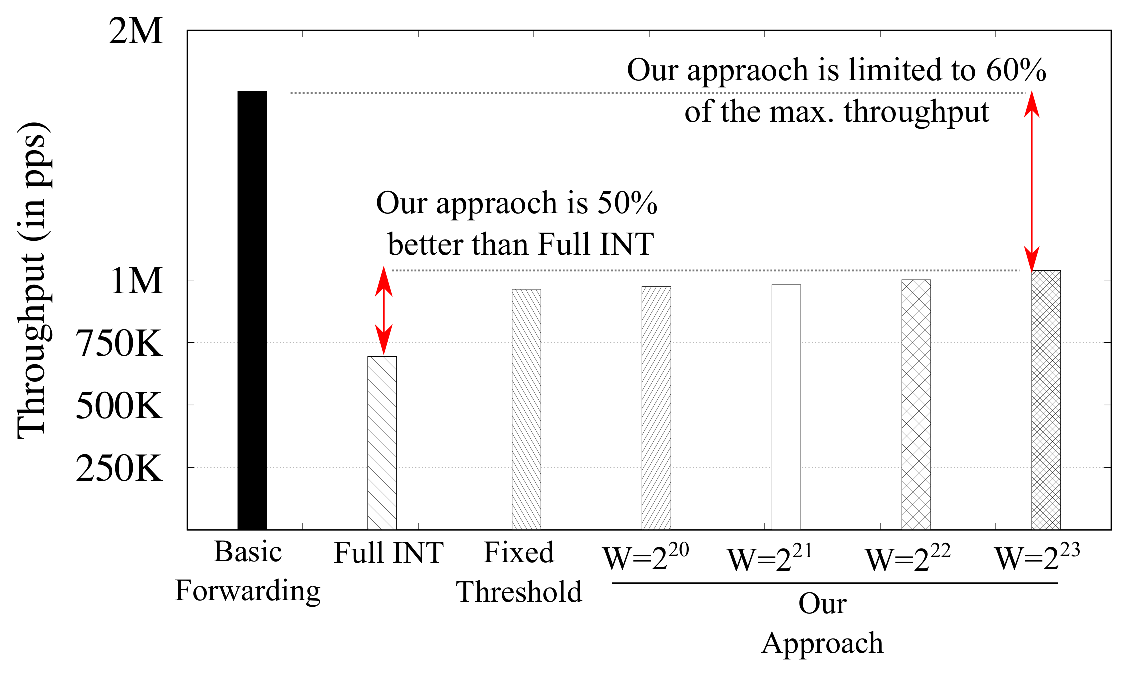
\includegraphics[scale=0.27]{results/g5-edited.eps}
            \label{fig-g5-a}
        }
\subfigure[Measured packet latency.]{
            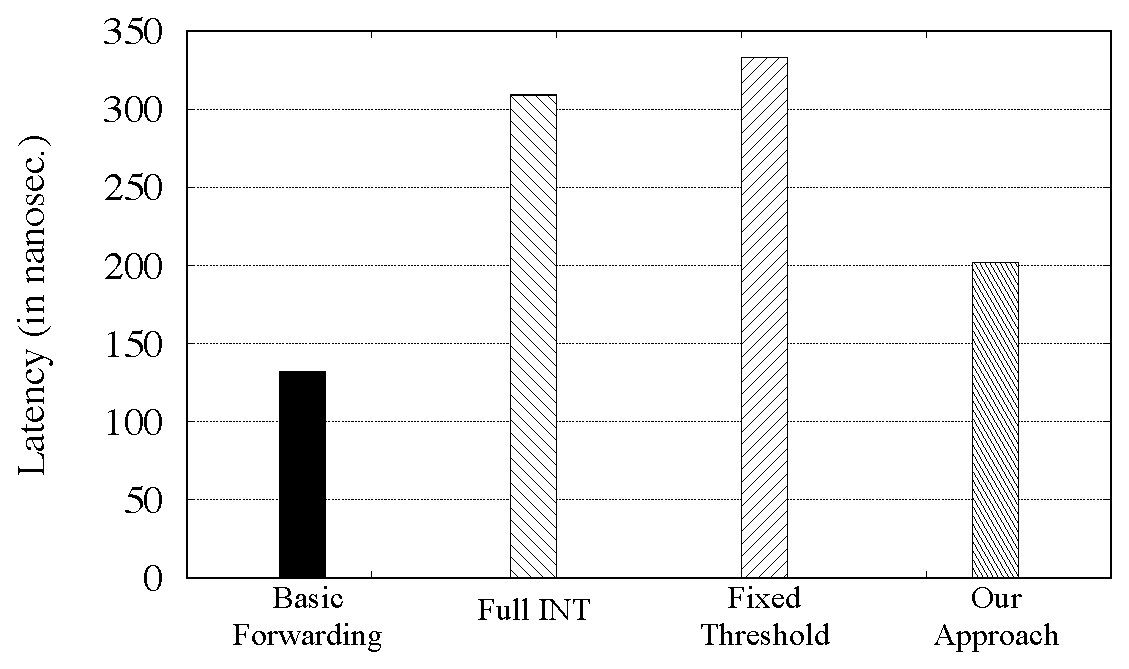
\includegraphics[scale=0.27]{results/g2.eps}
            \label{fig-g5-b}
        }
\caption{Impact of Throughput and Latency of our proposed approach.}
  \label{fig5}
\end{figure}




\section{Related Work}
The data plane programmability has opened up a wide range of research opportunities to solve existing network monitoring problems such as packet priorization~\cite{tr19_p4_int_vnf}, the usage of selective telemetry to reduce the network overload~\cite{tr18_selective_in-band}, and the classification and analysis of network flows~\cite{tr19_flowstalker}. As previously mentioned, INT allows the network flow packets to embed network telemetry data - such as in \cite{tang2019sel,ben2020pint,tr21_lint}.
%
Sel-INT~\cite{tang2019sel} leverages select group tables to selectively insert INT headers into software switches based on its bucket's weight and a certain probability.
%
Similarly, PINT~\cite{ben2020pint} leverages global hash functions and randomly decides to embed INT data in a given packet,
%
while LINT~\cite{tr21_lint} implements a mechanism with adaptive telemetry accuracy, where each node in the network analyzes its impact and decides whether to send the information to the collector.

P4Entropy~\cite{tr20_estimating_log} calculates the entropy of traffic by using the information contained in the packets. The entropy results are forwarded to the controller for storage and future analysis. Lin~et~al.~\cite{tr21_network_telemetry_by} perform data collection to allow the SDN controller to evaluate the behavior of network traffic to improve data routing.
%
Likewise, \cite{tr20_multi-feature} proposes a DDoS schema entirely in the data plane. It leverages typical DDoS metrics such as incoming flows and packet symmetry ratio and periodically triggers alarms to external controllers.

With the emergency of hardware technologies such as SmartNICs and domain-specific programming languages such as P4, more applications are being implemented directly in the data plane. The implementation of selective and dynamic monitoring with the use of additional headers~\cite{tr19_sampling-based}, the classification of packets into classes with the implementation of machine learning algorithms~\cite{tr19_do_switches_dream} and the detection of flow events~\cite{tr20_flow_event} are some examples of programmatic packet header manipulation.
%
NIDS~\cite{tr20_anomaly_detection} consists of a machine learning-based anomaly detection algorithm for detecting anomalous packets and future error mitigation. %Likewise, \cite{tr20_detection_of_fog} analyzes and embeds telemetry data of interest to the applications.
SwitchTree \cite{tr20_switchtree} performs the implementation of the Random Forest algorithm in the data plane for packet analysis and decision-making while updating the rules at runtime. \cite{tr21_programmable_sw} and \cite{tr19_do_switches_dream, tr20_switchtree} present an implementation of machine learning models in the data plane using decision tree, and aim to generate network mapping for intrusion detection services.

Current research efforts in the INT domain (e.g., \cite{ben2020pint, tr21_lint, tang2019sel}) have mostly neglected the costs of reporting telemetry data to INT collectors. In fact, existing work have considered either a full report of information or a selective one based on static thresholds.
%
In this work, we aim to fill this gap and offload the decision process of reporting INT data into the SmartNIC data plane in a dynamically manner. We propose a lightweight in-network mechanism based on a window-based moving average with collected INT data as input.

%Current research efforts in the INT domain have mostly focused on using in-band telemetry as a way to solve network management and operations problems. implementing  mechanisms  to  to solve  only consider static telemetry reports to INT collectors.
%\vspace{-5mm}


\section{Final Remarks}

In this paper, we propose a lightweight in-network mechanism to selective report in-band network telemetry to INT collectors. Our approach is based on a window-based moving average and it is tailored to SmartNIC architectures. By evaluating our approach in a state-of-the-art SmartNIC, we showed that our approach can report up to 16X less reporting statistics to INT collectors, while introducing a negligible overhead in terms of latency (1.5X higher than the baseline pipeline). As future work, we intend to explore machine learning algorithms in the data plane to decide whether to report data or not. Also, we intend to explore other offloading alternatives so that the processing workload can be split up on different SmartNICs or in eBPF/DPDK approaches.

%coordenar a coleta de dados com as metricas no INT sink


%\textcolor{red}{TBD. In this paper, we performed an extensive performance evaluation of SmartNICs to understand and quantify existing limitations. We focus our evaluation on measuring the performance in terms of latency and throughput for a plethora of packet memory-intensive scenarios. We showed that the line-rate throughput is bounded by (i) the number of register operations (up to 10 operations), (ii) the number of multiple match+action tables user in the pipeline (up to 5), (iii) the number of cryptography operations (up to 10). As future work, we intend to build an analytical model that can accurately estimate the performance of P4 applications executing on SmartNICs.}

%\section*{Acknowledgements}

%This work was partially funded by the National Council for Scientific and Technological Development (CNPq 2018/427814), Foundation for Research of the State of Sao Paulo (FAPESP 2018/23092-1), and Foundation for Research of the State of Rio Grande do Sul (19/2551-0001224-1,19/2551-0001266-7). 

%This work was partially funded by National Council for Scientific and Technological Development (CNPq) (grant 427814/2018-9), São Paulo Research Foundation (FAPESP) (grant 2018/23092-1), Rio Grande do Sul Research Foundation (FAPERGS) (grants 19/2551-0001266-7,20/2551-000483-0, 19/2551-0001224-1)





%by means of a MILP model. The main idea consists of dynamically guiding the acquisition process of telemetry data using learning mechanisms. We showed that our proposed model can effectively collect the most important telemetry items and provide accurate network-wide visibility to monitoring applications. Our model outperforms state-of-the-art heuristics by a factor of 2.5x with respect to the number of spatial dependencies satisfied and by a factor of 8x when comparing the number of anomalies identified.

\section*{Acknowledgements}

%This work was partially funded by National Council for Scientific and Technological Development (CNPq 2018/427814), Foundation for Research of the State of Sao Paulo (FAPESP 2018/23092-1), and Foundation for Research of the State of Rio Grande do Sul (19/2551-0001224-1,19/2551-0001266-7). 

This work was partially funded by National Council for Scientific and Technological Development (CNPq) (grant 427814/2018-9), São Paulo Research Foundation (FAPESP) (grants 2018/23092-1, 2020/05115-4, 2020/05183-0), Rio Grande do Sul Research Foundation (FAPERGS) (grants 19/2551-0001266-7, 20/2551-000483-0, 19/2551-0001224-1, 21/2551-0000688-9).

\vspace{-6mm}

\bibliographystyle{splncs04}
\scriptsize
\vspace{-2mm}


\bibliography{sample}

\end{document}
